\documentclass[a4paper,10pt,twoside, openright]{book}
\usepackage[english]{babel}
%\usepackage[utf8]{inputenc}
\usepackage{indentfirst}
\usepackage{graphicx}
\usepackage{epigraph}
\usepackage{atlasphysics}
\usepackage{subfigure}
\usepackage{lineno}
\usepackage{setspace}
\newcommand{\AC}{\ensuremath{\text{A}_{\text{C}}}}
\newcommand{\formatGenerator}[1]{\textsc{#1}}
\newcommand{\mcnlo}{\formatGenerator{mc@nlo}}
\newcommand{\wjets}{\ensuremath{W+\mathrm{jets}}}
\providecommand{\abs}[1]{\lvert#1\rvert}
\newcommand{\dy}{\ensuremath{\Delta{}\abs{y}}}
\newcommand{\deta}{\ensuremath{\Delta{}\abs{\eta}}}
\newcommand{\mtt}{\ensuremath{m_{\ttbar{}}}}
\newcommand{\Nupup}{\ensuremath{N(\uparrow\uparrow)}}
\newcommand{\Ndodo}{\ensuremath{N(\downarrow\downarrow)}}
\newcommand{\Nupdo}{\ensuremath{N(\uparrow\downarrow)}}
\newcommand{\Ndoup}{\ensuremath{N(\downarrow\uparrow)}}

\linespread{1.2}                        %comando per impostare l'interlinea
\usepackage{feynmf}
\usepackage{psfrag}
\usepackage[usenames,dvipsnames,svgnames,table]{xcolor}
\definecolor{light-gray}{gray}{0.9}
\usepackage{pgf,pgfarrows,pgfnodes}

\newcommand{\nocontentsline}[3]{}
\newcommand{\tocless}[2]{\bgroup\let\addcontentsline=\nocontentsline#1{#2}\egroup}

%\usepackage{ulem} %sostituisce l'effetto sottolineatura all'effetto corsivo nel comando \emph{} e risolve il problema delle righe che non si spezzano

\usepackage{multirow}
\usepackage{enumerate}

\usepackage[hdivide={3cm, *, 3cm}, vscale=0.75, bindingoffset=1cm]{geometry}
\usepackage{chngpage}

\usepackage[margin=7pt,font=small,labelfont=bf]{caption}
%\usepackage[margin=10pt,font=small,labelfont=bf]{caption}
%\usepackage[format=hang,indention=-2cm,labelfont=bf]{caption}%per delle caption più carine
\usepackage{booktabs}
\usepackage{longtable}
%\usepackage{pdflscape} 
%\usepackage[pdftex]{lscape}
\usepackage{lscape}
\usepackage{slashed}

\usepackage{listings}
\lstset{language=C}

\hyphenation{ca-lo-ri-me-ter ca-lo-ri-me-ters}%serve per la sillabazione: tra parentesi 

\setlength{\headheight}{15pt}
\usepackage{pict2e}
%\usepackage{guit}

%\usepackage{natbib}
%\bibliographystyle{unsrt}
%\usepackage[babel]{csquotes}
%\usepackage[style=numeric,sorting=none]{biblatex}
%\bibliography{biblio}


%MATHS
\usepackage{amssymb}
\usepackage{amsmath}
\usepackage{latexsym}
\usepackage{amsthm}
 \newcommand{\sgn}{\mathop{\mathrm{sgn}}}
\usepackage{slashed}

%\usepackage[T1]{fontenc}
%\usepackage{microtype}

\usepackage{fancyhdr}
\pagestyle{fancy}

\usepackage{eso-pic}

\usepackage{url}
\usepackage[ps2pdf,bookmarks=true,bookmarksnumbered=false,% true means bookmarks in left window are numbered
bookmarksopen=false, % true means only level 1 are displayed.
colorlinks=true,linkcolor=webred]{hyperref}
%\usepackage[pdfborder={0 0 0 0}]{hyperref}
\definecolor{webgreen}{rgb}{0, 0.5, 0} % less intense green
\definecolor{webblue}{rgb}{0, 0, 0.5} % less intense blue
\definecolor{webred}{rgb}{0.5, 0, 0} % less intense red

%END OF PACKAGES

%per includere il frontespizio (ottenuto in pdf a parte)
\newcommand\BackgroundPic{
\put(0,0){
\parbox[b][\paperheight]{\paperwidth}{%
\vfill
\centering

\includegraphics[width=\paperwidth,height=\paperheight,
keepaspectratio]{smallstuff/frontespizio}%
\vfill
}}}



%per avere l'indice senza numeri di pagina
\makeatletter 
 \newcommand{\cleantableofcontents}{% 
   \clearpage\begingroup 
   \let\ps@plain\ps@empty\pagestyle{empty}% 
   \tableofcontents\clearpage\endgroup} 
 \makeatother

%per lo stile dei capitoli
\makeatletter
\def\thickhrulefill{\leavevmode \leaders \hrule height 1ex \hfill \kern \z@}
%chstyle
\def\@makechapterhead#1{%
  \vspace*{10\p@}%
  {\parindent \z@ 
    {\raggedleft \reset@font
      \scshape \@chapapp{} \thechapter\par\nobreak}%
    \par\nobreak
    \vspace*{30\p@}
    \interlinepenalty\@M
    {\begin{spacing}{1.1} \raggedright \huge \bfseries #1\end{spacing}}%
    %{\doublespacing \raggedright \huge \bfseries #1}%
    \par\nobreak
    \hrulefill
    \par\nobreak
    \vskip 90\p@
  }}
\def\@makeschapterhead#1{%
  \vspace*{10\p@}%
  {\parindent \z@ 
    {\raggedleft \reset@font
      \scshape \vphantom{\@chapapp{} \thechapter}\par\nobreak}%
    \par\nobreak
    \vspace*{30\p@}
    \interlinepenalty\@M
    {\begin{spacing}{1.1} \raggedright \huge \bfseries #1\end{spacing}}%
    \par\nobreak
    \hrulefill
    \par\nobreak
    \vskip 90\p@
  }}



\renewcommand{\chaptermark}[1]{\markboth{\thechapter. \ #1}{}}
\renewcommand{\sectionmark}[1]{\markright{\thesection.\ #1}}
\fancyhf{}
\fancyhead[LO]{\small \nouppercase{\rightmark}}
\fancyhead[RE]{\small \nouppercase{\leftmark}}
\fancyhead[RO , LE]{ \thepage}


\newif\ifIsINT  % false by default
\IsINTfalse



\begin{document}
\linenumbers

\frontmatter
% Inizio Numerazione Romana
%\pagenumbering{roman}

\begin{titlepage}
\begin{adjustwidth}{-4cm}{-3cm}
\AddToShipoutPicture*{\BackgroundPic}
\end{adjustwidth}
\end{titlepage}

\clearpage{\pagestyle{empty}\cleardoublepage}

\thispagestyle{empty}

\null\vspace{\stretch{1}}
\begin{flushright}
\textit{A tempi migliori}
\vspace{\stretch{1}}\null

\begin{minipage}{.8\textwidth}\footnotesize
\begin{description}
\item[Professore:]  Lei ha una qualche ambizione?
\item[Nicola:] Ma\dots Non\dots
\item[Professore:] E Allora vada via\dots Se ne vada dall'Italia. Lasci l'Italia finch\'e \`e in tempo. Cosa vuole fare, il chirurgo?
\item[Nicola:] Non lo so, non ho ancora deciso\dots
\item[Professore:] Qualsiasi cosa decida, vada a studiare a Londra, a Parigi\dots Vada in America, se ha le possibilit\`a, ma lasci questo Paese. L'Italia \`e un Paese da distruggere: un posto bello e inutile, destinato a morire.
\item[Nicola:] Cio\`e, secondo lei tra poco ci sar\`a un'apocalisse?
\item[Professore:] E magari ci fosse, almeno saremmo tutti costretti a ricostruire\dots Invece qui rimane tutto immobile, uguale, in mano ai dinosauri. Dia retta, vada via\dots
\end{description}

\begin{flushright}
\textit{da} La meglio Giovent\`u \textit{di M.T. Giordana (2003)}
\end{flushright}
%\`o \`o - à \`a - è \`e - ì \`i - ù \`u - é \'e


\end{minipage}
\end{flushright}


\clearpage{\pagestyle{empty}\cleardoublepage}

\clearpage{\pagestyle{empty}\cleardoublepage}

\chapter*{Introduccion}\label{chap:introES}



\clearpage{\pagestyle{empty}\cleardoublepage}

% Indice

\pdfbookmark[1]{Index}{Index}
\cleantableofcontents

% Elenco delle Figure
%\addcontentsline{toc}{section}{\listfigurename}
%\listoffigures

\clearpage{\pagestyle{empty}\cleardoublepage}

\phantomsection
\addcontentsline{toc}{chapter}{Introduction}
\clearpage{\pagestyle{empty}\cleardoublepage}

\chapter*{Introduction}\label{chap:intro}

%\vskip-2.5cm

%\subsection*{Part I}
July 4th, 2012, represents a milestone for high-energy physics,
being the date when the ATLAS and CMS experiments at CERN announced
the discovery of a new particle consistent with a Standard Model Higgs
boson with mass $m_H\sim 125\gev$. Is it going to be celebrated, 20 years
from now, as the beginning of a new era of discoveries or as the 
end of the adventure? Is there something {\it more}, out there, in 
the outer space or 100~m underground, awaiting for being discovered?
As outlined in Chapter~\ref{chap:TH} there is quite some evidence
something must be there lying ``beyond the Standard Model''. 
A successful theory finally completed
by the identification of the Higgs boson, 
the Standard Model as it is still leaves too many questions
unanswered. What is ``Dark Matter'', this exotic form of energy density different
from atoms, being immune to electromagnetic interactions, but which
is known to account for $\sim$27\% of the total matter in the Universe?
After the Big Bang, what caused the asymmetry in the production of particles vs
antiparticles that made matter prevail over antimatter?
Why is the top quark so much heavier than the other quarks? Why is the
Higgs boson so much lighter than the Planck mass?

It was to find an explanation to this puzzle that the 
Large Hadron Collider project was initiated 20 years ago. The ATLAS
collaboration then started the design of the detector described in
Chapter~\ref{chap:atlas}, outlining an ambitious physics program
in which the search for the Higgs boson was ``just'' the first bullet
of the list.
The LHC first run was on the 20th of November 2009, with the ATLAS
experiment beginning to record data from these early proton-proton
collisions at a \cme\ of $900$~GeV just three days later.
Since then, outstanding performances of both the accelerator
and the detector allowed to collect a huge amount of data
from proton-proton collisions at increasing center of mass energies, reaching in
2012 a total of $\sim$20~\ifb\ at a \cme\ of 8~TeV.

%During the long time that passed between the detector construction
%and when the real data became available in 2009, analyses relied on
%data collected during test-beam runs and on Monte Carlo simulation.
However, this large amount of data alone would 
not tell much if it were not possible to
compare them to precise theoretical predictions.
Chapter~\ref{chap:mc} describes the Monte Carlo techniques used
to obtain simulated samples of either ``Standard Model'' %processes 
or ``new physics'' events. 
%Monte Carlos are powerful tools that used with the purpose of 
%calibrating the detector, 
%modeling the contributions to some particular channel
%allow 
Starting from the computation of the matrix element of a 
particular process, Monte Carlo tools
are combined to obtain the complete picture of how the
event of interest develops, including as a last step
the simulation of the particles interactions with the
detector material.

Whether real data or Monte Carlo simulated samples, at
the ``raw'' level events are simple digital outputs, coming respectively
from the real or simulated response of the read-out electronics
of the different ATLAS detector subsystems. How these outputs
are assembled into physical objects is described in Chapter~\ref{chap:objects},
where the reconstruction process is explained.
The outcome is a dataset containing all the information needed
about physics objects such as leptons, jets and energy 
imbalance of the event,
ready to be processed by analyses.


%\subsection*{Part II}
%The object of this dissertation is then introduced in Chapter~\ref{chap:vlq}.
Using these kind of datasets, 
%motivated by more than one theoretical proposals for beyond Standard Model physics, 
the Exotics group of the ATLAS collaboration defined a search strategy 
for exotic heavy quarks different from the first three generations 
%in that they do not show a chiral behavior under the electroweak group transformations.
%These quarks are 
and called ``vector-like''. Even though these quarks are
predicted in various proposed extentions of the Standard Model, 
like extra-dimensions or composite Higgs
models, no details on their masses are given and their decay branching fractions
are very model dependent. Searches aiming at inclusivity 
must therefore rely as little as possible on 
assumptions from the model, and this is the approach chosen for the
two searches in the single lepton channel
for pair-produced heavy vector-like top partners 
presented in this dissertation. The general quasi-model independent
strategy common to the two analyses, performed analyzing 
$\sim$14~\ifb\ of data from proton-proton collisions at the
 \cme\ $\rts=8\tev$ recorded during the year 2012 
at the ATLAS experiment, is presented in
Chapter~\ref{chap:vlq}.

The search for pair-produced heavy vector-like top partners
where at least one of them decays into a $W$ boson and a bottom
quark is detailed in Chapter~\ref{chap:wbx}. The key point in
this analysis is the reconstruction of the $W$ boson from its
hadronic decay products which allows for the reconstruction
of the heavy quark mass, a very good discriminating variable between
signal and Standard Model background processes.

Chapter~\ref{chap:htx} presents the search for 
pair-produced heavy vector-like top partners
where at least one of them decays into a Standard Model Higgs
boson and a top quark. In this case the main decay of the Higgs
boson into two bottom quarks is exploited resulting in a
final state signature characterized by a high number of recontructed
jets, where a large fraction of them is identified as originating
from the hadronization of bottom quarks.

While the individual results from the searches
are presented in the respective chapters, higher
sensitivity is achieved combining the two analyses.
This is described in Chapter~\ref{chap:results},
and the result of these searches is compared with
other similar searches exploiting multi-lepton signatures.
%where also a prospect is given of a potential combination of these searches with the other analyses performed by ATLAS searching for heavy vector-like quarks in final states with two leptons.






%\newpage
%\phantomsection
%\addcontentsline{toc}{section}{Acknowledgement}
\subsubsection*{Personal contributions and acknowledgement}

The results presented in this dissertation represent
a small sample of the achievements made possible by
the combined effort of many, many people. The ATLAS
collaboration itself consists of $\sim$3000 scientists,
working in different subgroups. In particular,
the author of this dissertation participated to calibration
and performance studies of the hadronic calorimeter
and to the improvement of data-driven estimation of
multi-jet backgrounds for analyses with top quarks 
decaying in the single-muon channel. Regarding
the two analyses object of this dissertation, the author
has been amongst the main analyzers, implementing and
running the signal selection and statistical analysis and
performing the needed cross checks for the good modeling
of background predictions. % and for Monte Carlo signal modeling.
The results are documented in two preliminary 
notes~\cite{ATLAS-CONF-2013-060,ATLAS-CONF-2013-018}.
The work for the final analyses to be published is still on-going at
the time of the writing of this dissertation.
The author also significantly participated to a previous,
published analysis~\cite{ATLAS:2012qe}
performed on the data from lower \cme\ 
proton-proton collisions which pioneered searches for
heavy vector-like quarks in ATLAS.

A particular acknowledgement goes to the ``IFAE-top''
group, present and former members, for their fundamental
contributions to the common analysis framework used
for these searches.


\clearpage{\pagestyle{empty}\cleardoublepage}


\mainmatter



\section{Going beyond the SM with vector-like quarks}\label{sec:THvlq}

\cite{AguilarSaavedra:2009es,Martin:2009bg}

\subsection{Production}\label{sec:vlqprod}


\subsection{Decay}\label{sec:vlqdecay}





\clearpage{\pagestyle{empty}\cleardoublepage}
\clearpage{\pagestyle{empty}\cleardoublepage}

\chapter{The ATLAS experiment at the Large Hadron Collider}\label{chap:atlas}

The analyses presented in this dissertation have been performed analyzing data from 
proton-proton (p-p) collisions at the \cme $\rts=8\tev$ recorded during the year 2012 
at the ATLAS experiment~\cite{Aad:2008zzm}. In the following Chapter we will briefly 
describe the main features of the detector, located at the CERN laboratories in Geneva,
Switzerland.

The experimental facilities are situated at Point~1 along the Large Hadron Collider 
(LHC)~\cite{lhc} 27~km long ring, shown in Figure~\ref{fig:lhcring}. The accelerator
tunnel can reach an underground depth of 175~meters and is spread between Swiss
and French territory, while the cave where ATLAS is allocated is about 100~meters 
underground in the CERN Swiss site of Meyrin. 

\begin{figure}[tb]\begin{center}
	\subfigure{\label{fig:lhcring}
  	\includegraphics[width=0.8\textwidth]{detector/figures/ring.eps}}
	\caption{A schematic showing the accelerator complex at CERN. Protons are
        extracted from Hydrogen gas and injected in the first machine, the linear 
        accelerator LINAC2 that starts the acceleration chain. When protons reach
        an energy of 50\mev they are injected into the Proton Synchrotron Booster
        (PSB) and accelerated up to the energy of 1.4\gev. The second circular
        accelerator, the Proton Synchrotron (PS) brings the energy of the protons
        to 25\gev previous to injecting them into the last machine before the LHC,
        the Super Proton Synchrotron (SPS). Protons of 450\gev finally enter the
        LHC where they are boosted to energies of up to 4\tev.
        The four main LHC experiments are shown on the collider ring.}
\end{center}\end{figure}

The LHC program was approved by CERN Council in 1994, followed by the approval of
the four main experiments physics programs: ATLAS~\cite{Aad:2008zzm} and CMS~\cite{cms}
in 1996; ALICE~\cite{alice} in 1997; LHCb~\cite{lhcb} in 1998.
Works towards the installation of the most powerful particle accelerator of the world
started when the Large Electron Positron Collider (LEP) was dismantled in 2000 to 
give up its place in the tunnel to the LHC, which was then fully operational by 2008.

The LHC is composed of eight arcs 2.7~km long, each of which contains 154 dipole 
magnets, whose function is to  bend the beams along the circular trajectory, and
49 quadrupole magnets, that focus the beam. These superconducting magnets operate
at a temperature of 1.9~K, maintained by means of liquid Helium vessels.
Eight insertions are placed inbetween the arches. Each insertion has a specific
role that characterizes its design and can be injection, beam dumping, beam cleaning,
or ``physics'', i.e. make the beams collide within an experiment.

First proton beams were circulated on 10th September 2008 and right on the verge of
getting the first collisions at a \cme $\rts=900\gev$ nine days later, an electrical
connection joining superconducting wires of a dipole and a quadrupole
failed. This caused the release of liquid Helium in the insulating vacuum,
resulting in an explosion that severely damaged the machine.
After more than one year devoted to repair the damage and consolidate the security,
on 30th November 2009 the LHC became the world's highest energy particle 
accelerator\footnote{\url{http://press.web.cern.ch/press/PressReleases/Releases2009/PR18.09E.html}}:
\begin{quotation}\small
Geneva, 30 November 2009. CERN's Large Hadron Collider has today become the world’s highest energy particle accelerator, having accelerated its twin beams of protons to an energy of 1.18 TeV in the early hours of the morning. This exceeds the previous world record of 0.98 TeV, which had been held by the US Fermi National Accelerator Laboratory’s Tevatron collider since 2001. It marks another important milestone on the road to first physics at the LHC in 2010.
\end{quotation}





The main performance figure of merit for an accelerator is the luminosity, the 
instantaneous luminosity $\mathcal L$ being defined as 
\begin{equation}\label{eq:lumiN}
\mathcal{L}\times\sigma=\dfrac{dN}{dt}=f\times n\dfrac{N_1\times N_2}{A}\times\sigma.
\end{equation} 
Here $dN/dt $ is the event rate of a certain process and $\sigma$ is its cross 
section. This rate is directly proportional to the the frequency $f$, the number 
of bunches $n$ and the number of particles in the two bunches $N_1, N_2$, and
inversely proportional to the beam cross-section $A$.

Integrating over the accelerator active time (a ``fill'', when stable beams are kept
colliding) gives the \textit{integrated luminosity}, relating the total number 
of produced events $N_{tot}$ to the cross-section:
\begin{equation}\label{eq:intLumi}
\int \mathcal L dt  = \dfrac{N_{tot}}{\sigma} 
\end{equation}


\clearpage{\pagestyle{empty}\cleardoublepage}
\clearpage{\pagestyle{empty}\cleardoublepage}

\chapter{Monte Carlo simulation}\label{chap:mc}


\section{Parton shower}\label{sec:partonshower}

\section{Hadronization}\label{sec:hadronization}

\section{Underlying-event}\label{sec:underlyingevent}

\section{Generators}\label{sec:generators}



\clearpage{\pagestyle{empty}\cleardoublepage}
%\clearpage{\pagestyle{empty}\cleardoublepage}

%\chapter{Object reconstruction}\label{chap:objects}
\section{Object reconstruction}\label{chap:objects}

After having described the ATLAS detector, in the following Section we will
explain how object (electrons, muons, jets and the missing transverse energy \met) 
are reconstructed to be used in physics analyses. In addition details from
selections common to the analyses presented in this dissertation are given.


%\section{Electrons}\label{sec:electrons}
\subsection{Electrons}\label{sec:electrons}
Electrons are reconstructed for pseudorapidities up to $|\eta| = 2.5$, where
information from the ID is available, matching a track with an energy deposit
(cluster) in the electromagnetic calorimeter. 

To identify tracks from ID points an inside-out algorithm is used, starting from a 
seed of three aligned hits in the pixel detector or in the SCT. Five fundamental parameters,
shown and described in Figure~\ref{fig:trackpar}, are computed and used for the subsequent 
steps of hits association. The candidate track must be 

\begin{figure}[tb]\begin{center}
	\subfigure[]{
  	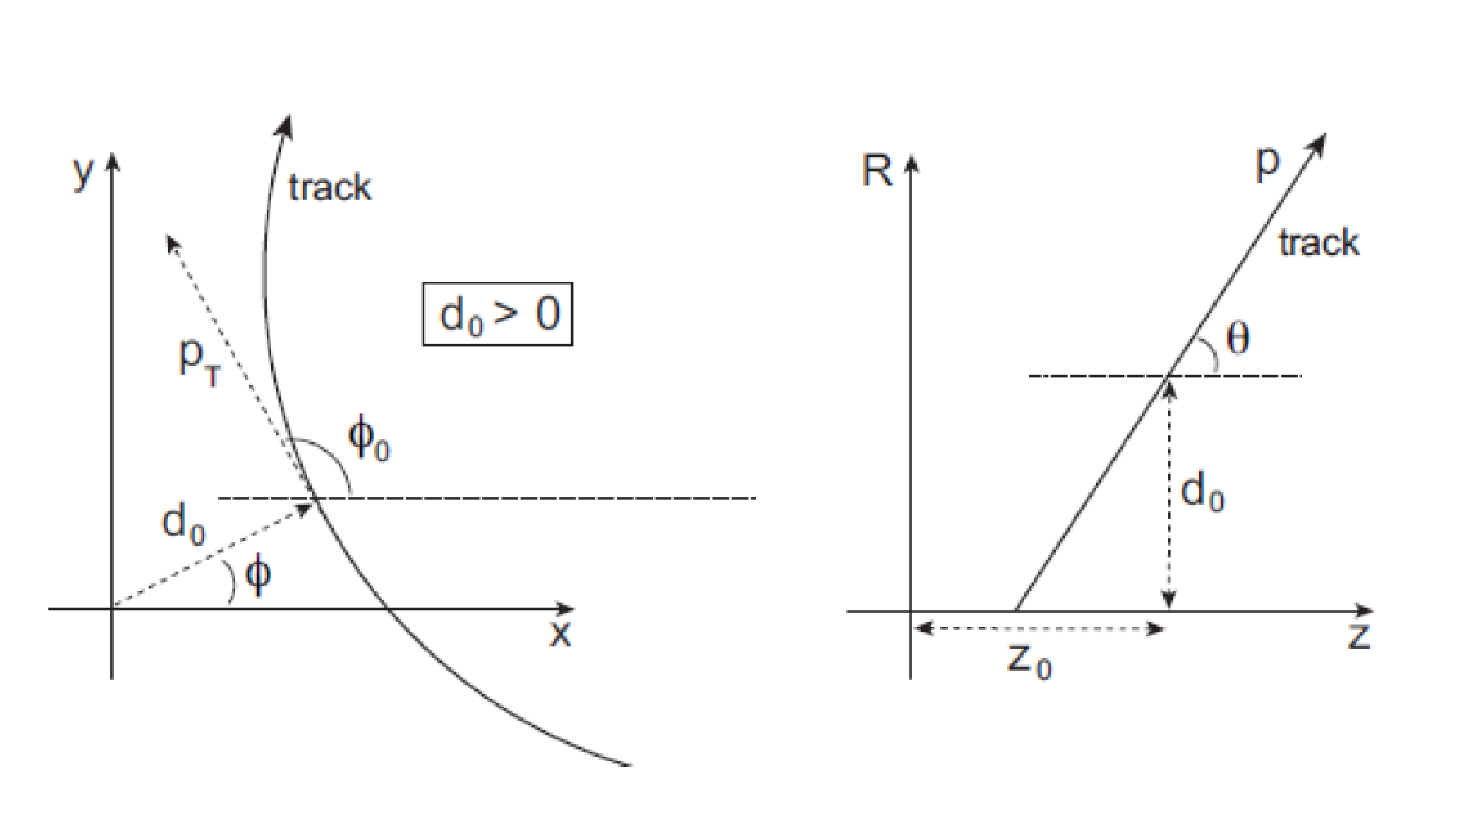
\includegraphics[width=0.7\textwidth]{objectsreconstruction/figures/tracks}}
	\caption{Schematic drawings of the parameters used for track reconstruction in the XY and $R$Z planes (left and right respectively).
          The parameters are: $q/p$, the charge divided by the momentum; $\theta$, or more used $\eta$, the angle
          with respect to the Z axis in the $R$Z plane measured from the perigee; $\phi_0$, the angle 
          with respect to the X axis in the XY plane measured from the perigee; $d_0$, the impact parameter, 
          or perigee with respect to the Z axis in the XY plane; $z_0$, Z component of the perigee.\label{fig:trackpar}}
\end{center}\end{figure}


Clusters are built starting from
$\Delta\eta\times\Delta\phi=0.025\times0.025$ single energy deposits summing
up into towers. Adjacent towers form clusters of $3\times7$ cells units in $\eta\times\phi$
in $|\eta|<1.4$ and $5\times5$ further.




excluding the transition region $1.37<|\eta| <1.52$
with inactive material.



%\section{Muons}\label{sec:muons}
\subsection{Muons}\label{sec:muons}



%\section{Jets}\label{sec:jets}
\subsection{Jets}\label{sec:jets}


%\section{Missing Transverse Energy}\label{sec:met}
\subsection{Missing Transverse Energy}\label{sec:met}


\clearpage{\pagestyle{empty}\cleardoublepage}
\clearpage{\pagestyle{empty}\cleardoublepage}

\chapter{Searches for vector-like top partner pairs in the single lepton channel}~\label{chap:vlq}

In the following Chapter we will describe two searches for vector-like 
top partners \TTbar\ pairs performed in the single 
lepton\footnote{From now on, with the word ``lepton'' we will 
mean only either electron or muon, assumed to come from the leptonic
decay of a $W$ boson with its associated neutrino, which is considered
to be the only particle contributing to the transverse missing energy \met.} channel. 
These analyses
are optimized for different final states and are thus complementary.
The first search focuses on decay channels with high BR to $Wb$ and is 
performed using the full dataset of p-p collisions at the \cme of \rts=8~\tev\
collected during 2012 at the ATLAS detector, consinsting in 20.34~\ifb, while
the preliminary search for vector-like top partners with high BR to $Ht$
uses a partial dataset of the same data, amounting to 14.3~\ifb.

The Chapter is organized as follows: first Section~\ref{sec:presel}
introduces the common event preselection for data and few general concepts in the
analyses design; Section~\ref{sec:MCbkg}
presents the Monte Carlo samples used in the searches, which
are in general common to both analyses with only few exceptions that are reported;
Section~\ref{sec:qcdbkg} describes how the multi-jet background from QCD events is
obtained.
Finally, the two analyses are detailed in Section~\ref{sec:wbx} and Section~\ref{sec:htx}, 
which illustrate the event selection criteria, the background modeling estimation, 
the systematics affecting the analysis, the statistical treatment and the
results.

\section{Data sample and common event preselection}\label{sec:presel}

The data from p-p collision events recorded at the ATLAS experiment during
2012 at a \cme\ of $\rts=8\tev$ are considered. Physics object definitions 
were previously discussed in Section~\ref{sec:objects}.
Events collected during
stable beam periods are required to pass data quality requirements and
single lepton trigger selection. In order to maximize trigger
efficiency, different transverse momentum threshold triggers are combined
through a logical \OR, with the lower \pt\ ones including isolation requirements
that result in inefficiencies for high \pt\ lepton candidates, recovered with
the use of the higher threshold triggers. The electron triggers have
\pt\ thresholds of 24 and 60\gev, the muon ones of 24 and 36\gev.

After passing trigger requirements, events with more than one lepton are
discarded. In addition, the only lepton of the event has to match within $\dr<0.15$ the
triggered one. As basic preselectio, four jets satisfying the conditions
described in Section~\ref{sec:jets} are required, at least one of them
being tagged as a \bjet.

In order to suppress the multi-jet background from QCD processes,
combined cuts on the \met\ and on the tranverse mass of the 
leptonically decaying $W$ boson \mt\footnote{$\mt = \sqrt{2 p^\ell_{\rm T} \met (1-\cos\Delta\phi)}$, with
$p^\ell_{\rm T}$  being the transverse momentum (energy) of the muon (electron) and $\Delta\phi$ the
azimuthal angle separation between the lepton and the direction of
the missing transverse momentum.}\ 
are defined: $\met>20~\gev$ and $\met+\mt>60~\gev$.

At this point, a simple consideration about the typical expected jet
(and \bjet) multiplicity is made so as to define an orthogonality
cut between the two analyses. Table~\ref{tab:jetmult} shows the 
number of jets (\bjet s) per decay channel combinations of \TTbar\ pairs, 
in the case of single lepton selection with at least four jets
(i.e. one $W$ boson will always decay into lepton and neutrino,
and $Z$ boson decay to neutrinos is excluded in the $WbZt$ channel) and assuming that
the Higgs boson decays to a bottom quark-antiquark pair.
To avoid overlap between selected events from the two analyses, in the
\wbx\ analysis events with $\geq$6 jets and $\geq$3 \bjet s are 
rejected\footnote{As will be explained later in Section~\ref{sec:htxEVT}, another orthogonality
cut will be applied in the low \bjet\ multiplicity channel of the \htx\ analysis.}.

\begin{table}\centering
	\begin{tabular}{lccc}\toprule
	 & $Wb$ & $Ht$ & $Zt$ \\\midrule
             &\cellcolor{lightgray} & & \cellcolor{lightgray}\\
	\multirow{-2}{*}{$Wb$} & \cellcolor{lightgray}\multirow{-2}{*}{\bf 4 (2)} & \multirow{-2}{*}{6 (4)} & \cellcolor{lightgray}\multirow{-2}{*}{{\bf 6} ({\bf2}/4)} \\
        \multirow{2}{*}{$Ht$} & \multirow{2}{*}{6 (4)} & \multirow{2}{*}{8 (6)} & max: 8 (4/6)\\
             & & & \cellcolor{lightgray}min: {\bf6 (2)}\\
        \multirow{2}{*}{$Zt$} & \cellcolor{lightgray}& max: 8 (4/6) & \cellcolor{lightgray}max: {\bf8} ({\bf2}/6) \\
             & \cellcolor{lightgray}\multirow{-2}{*}{\bf6 (2/4)} & \cellcolor{lightgray}min: {\bf6 (2)} & \cellcolor{lightgray}min: {\bf6} ({\bf2}/4)\\
	\bottomrule\end{tabular}\caption{Jets (\bjet s) multiplicities in the various possible final states. $Z$ boson decays 55\% hadronically, 15\% of the 
        times into \bbbar, therefore the min/max number of \bjet s is reported. Highlighted are the channels that after the orthogonality cut
        will contribute to the \wbx\ analysis.}\label{tab:jetmult}
\end{table}




\section{Background and signal modeling}\label{sec:datasets}

The main background for both analyses is $t\bar{t}$ 
production with jets ($t\bar{t}$+jets in the following) 
and different choices for the generator are made
in the analyses because of the specific needs of having well
modeled regions.
In the case of the $t\bar{t}$+jets background prediction for the \htx\ analysis 
further corrections to match the data are applied, due to a mismodeling in the
heavy- and light-flavour content of the simulated sample (see Section~\ref{sec:htxEVT}).

$W$ boson production  in association with jets ($W$+jets in the following) 
and multi-jet events from QCD processed also contributes, the latter
sneaking into the event selection via the misidentification of a jet or a photon as an
electron or the presence of a non-prompt lepton from, e.g., semileptonic $b$- or $c$-hadron decay.
Other background smaller components are single top quark, $Z$+jets, diboson
($WW,WZ,ZZ$), and $t\bar{t}$ production associated with a vector or Higgs boson.

All event generators using {\sc Herwig}~\cite{herwig} are also interfaced to {\sc
Jimmy} v4.31~\cite{jimmy} to simulate the underlying event.  
With the exception of the 
signal samples, all simulated 
samples utilise {\sc Photos 2.15}~\cite{PhotosPaper} to model
photon radiation and {\sc Tauola 1.20}~\cite{TauolaPaper} to model
$\tau$ decays.  

All simulated samples include multiple p-p
interactions and go through the  {\sc Geant4}~\cite{geant}
detector geometry and response simulation~\cite{atlas_sim}
with the exception of the signal samples, for which a fast simulation of
the calorimeter response is used.

All simulated samples are then processed through the same reconstruction 
software as the data and are reweighted to match 
the instantaneous luminosity profile in data. 

%Additional corrections are applied so that the 
%object identification efficiencies, energy
%scales and energy resolutions match those determined in data control
%samples.


\subsection{Monte Carlo simulated samples}\label{sec:MCbkg}

\subsubsection{$t\bar{t}$ MC@NLO}\label{subsec:MC@NLO}
Simulated samples of $t\bar{t}$ pair production  in association with jets 
($t\bar{t}$+jets or simply $t\bar{t}$ in the following)
are generated with {\sc MC@NLO} v4.01~\cite{mcatnlo_1,mcatnlo_2,mcatnlo_3} using the {\sc CT10} set of parton distribution functions (PDFs)~\cite{ct10},
with the parton-shower and fragmentation steps being performed by 
{\sc Herwig} v6.520~\cite{herwig}.
The top quark mass is assumed to be equal to $172.5\gev$ and 
the samples are normalized to approximate next-to-next-to-leading-order 
(NNLO) theoretical cross section~\cite{ttbarxs}; the cross section used 
has been computed with {\sc Hathor} 1.2~\cite{ttbarxs} using the {\sc MSTW2008}
NNLO PDF set~\cite{mstw} and is $\sigma_{t\bar{t}}= 238^{+22}_{-24}$~pb, 
where the total uncertainty results from the sum in quadrature of the 
scale and PDF+$\alpha_S$ uncertainties according to 
the {\sc MSTW} prescription~\cite{mstw2}. 
This is the $t\bar{t}$ used in the \wbx\ analysis.

\subsubsection{$t\bar{t}$ Alpgen}\label{subsec:alpgen}
Simulated samples of $t\bar{t}$+jets are generated using
%and $W/Z$+jets events are generated using
 the {\sc Alpgen v2.13}~\cite{alpgen} leading-order (LO) generator and the 
{\sc CTEQ6L1} PDF set~\cite{cteq6}, with parton shower and fragmentation  
modelled through {\sc Herwig} v6.520~\cite{herwig}.

A parton-jet matching scheme called ``MLM matching''~\cite{mlm} is used
in orderd to avoid double-counting  of partonic configurations
eventually generated both at the matrix-element calculation level
and at the parton-shower evolution step.

Separate samples are generated for $t\bar{t}$+light jets ($t\bar{t}$+light 
or $t\bar{t}$+LF in the following, from ``light flavour'') 
with up to three additional light partons ($u$, $d$, $s$ quarks or gluons),
and for $t\bar{t}$+heavy-flavour jets ($t\bar{t}$+HF in the following), 
including $t\bar{t}b\bar{b}$ and
$t\bar{t}c\bar{c}$.  
An algorithm based on the angular separation
between the extra heavy quarks is used to remove 
the overlap between $t\bar{t}q\bar{q}$ ($q=b,c$) 
generated from the matrix element calculation and 
from parton-shower evolution in the  $t\bar{t}$+light samples
is employed: matrix-element prediction is chosen over the parton-shower one
when $\Delta R(q,\bar{q})>0.4$, else vice-versa.

%The algorithm used is implemented in the HFOR tool~\cite{hfor}.

Again a top quark mass of $172.5\gev$ is assumed, and normalisation to the
NNLO theoretical cross section is used (see~\ref{subsec:MC@NLO})

\subsubsection{$W/Z$+jets}

Simulated samples of $W/Z$ boson production in association with jets
($W/Z$+jets in the following) are generated with up to five additional 
partons using the {\sc Alpgen v2.13}~\cite{alpgen} LO generator and the 
{\sc CTEQ6L1} PDF set~\cite{cteq6}, interfaced to {\sc Herwig} v6.520 
for parton showering and fragmentation.

``MLM matching'' is used also here to avoid double-counting of partonic configurations 
between  matrix-element  calculation and parton showering.

The $W$+jets samples are generated separately for $W$+light jets, 
$Wb\bar{b}$+jets, $Wc\bar{c}$+jets, and $Wc$+jets, 
with the relative contributions normalized using the fraction 
of $b$-tagged jets in $W$+1-jet and $W$+2-jets data 
control samples~\cite{whf}, while
the $Z$+jets samples are generated separately 
for $Z$+light jets, $Zb\bar{b}$+jets, and $Zc\bar{c}$+jets and
normalized to the inclusive NNLO theoretical cross section~\cite{vjetsxs}.

Overlap between $W/Zq\bar{q}$+jets ($q=b,c$) 
events generated from the matrix element calculation and those
generated from parton-shower evolution in the $W/Z$+light jets
samples is avoided via an algorithm analogous to the one used
for $t\bar{t}$ Alpgen.

For the $W$+jets background, a normalisation from data for the shapes 
obtained from the simulation is derived since the simulation 
overestimates the number of $W$+jets events
by up to $\sim$20\%, depending on the jet multiplicity.

By exploiting the predicted asymmetry between
$W^+$+jets and $W^-$+jets production in p-p collisions~\cite{wasym},
the total number of $W$+jets events in data ($N_W=N_{W^+}+N_{W^-}$), 
can be estimated based on the measured
difference between the number of positively- and negatively-charged $W$
bosons, $(N_{W^+}-N_{W^-})_{\rm meas}$, and the asymmetry predicted from the simulation:
\begin{equation}
N_W = \left(\frac{N_{W^+}+N_{W^-}}{N_{W^+}-N_{W^-}}\right )_{\rm MC}(N_{W^+}-N_{W^-})_{\rm meas}
\label{eq:nw}
\end{equation}

Events are categorised in terms of  multiplicity of $b$ and $c$ jets and scale factors are
derived using Equation~\ref{eq:nw}.
The fraction of $W$+light jets events is scaled accordingly
in order to preserve the overall normalisation of the $W$+jets background before $b$ tagging.


\subsubsection{Other backgrounds}\label{subsec:otherbkg}
%,tchanxs,Wtchanxs,schanxs}. 
Simulated samples of single top quark backgrounds corresponding to the
$s$-channel and $Wt$ production mechanisms are generated with {\sc
MC@NLO} v4.01~\cite{mcatnlo_1,mcatnlo_2,mcatnlo_3} using the {\sc
CT10} PDF set~\cite{ct10}.  In the case of $t$-channel single top
quark production, the {\sc AcerMC} v3.8 LO generator~\cite{acermc}
with the {\sc MRST LO**} PDF set is used.

Simulated samples of $t\bar{t}$ produced in association with a $W$ or $Z$ boson
($t\bar{t}V$ $(V=W,Z)$ in the following) are generated with the {\sc Madgraph v5} LO
generator~\cite{madgraph} and the {\sc CTEQ6L1} PDF set.  

Samples of $t\bar{t}$ produced in association with a Higgs boson
($t\bar{t}H$ in the following) are generated with the 
{\sc Pythia} 6.425~\cite{py6} LO generator and the {\sc MRST LO**} PDF set~\cite{mrst},
assuming a Higgs boson mass of $125\gev$ and considering the 
$H\to b\bar{b}$, $c\bar{c}$, $gg$, and $W^+W^-$ decay modes.

Parton shower and fragmentation are modelled with {\sc Herwig}
v6.520~\cite{herwig} in the case of {\sc MC@NLO}, with {\sc Pythia}
6.421 in the case of {\sc AcerMC}, and with {\sc Pythia} 6.425 in the
case of {\sc Madgraph}.  All these samples are generated assuming a top
quark mass of $172.5\gev$. The single top quark samples are normalised to
the approximate NNLO theoretical cross sections~\cite{stopxs,stopxs_2}
using the {\sc MSTW2008} NNLO PDF set, while the $t\bar{t}V$ samples
are normalised to the NLO cross section predictions~\cite{ttbarVxs1,ttbarVxs2}.
The $t\bar{t}H$ sample is normalised using the NLO theoretical cross section 
and branching ratio predictions~\cite{lhcxs}.
Finally, the diboson backgrounds are modelled using {\sc Herwig} with
the {\sc MRST LO**} PDF set, and are normalised to their NLO
theoretical cross sections~\cite{dibosonxs}.

\subsubsection{Signal samples}\label{subsec:MCsignal}


For vector-like $T$ signals, samples corresponding to a singlet $T$ quark 
decaying to $Wb$, $Zt$ and $Ht$ are generated with the {\sc Protos} v2.2 
LO generator~\cite{jaas,protos} 
using the  {\sc MSTW2008} LO PDF set, and interfaced to {\sc Pythia} for 
the parton shower and fragmentation. 

For each decay channel ($Wb$, $Zt$ and $Ht$) the branching ratio has been 
set to 1/3. Events are reweighted
in order to reproduce any desired branching ratio configuration. 

The predicted branching ratios in the weak-isospin singlet and doublet scenarios as 
a function of $m_{T}$ are given in Table~\ref{tab:BRT}.

The $m_{T}$ values considered range from $350\gev$ to $850\gev$ in steps of $50\gev$, 
with the Higgs boson mass assumed 
to be $125\gev$. All Higgs boson decay modes are considered, 
with branching ratios as predicted by {\sc hdecay}~\cite{hdecay}.

Signal samples are normalized to the approximate NNLO theoretical cross sections~\cite{ttbarxs} using the {\sc MSTW2008} NNLO PDF set.
The cross section values used are summarized in Table~\ref{tab:sigmaTT}.



\begin{table}[h!]
\begin{center}
\begin{tabular}{c c c c c c c}
\hline
\hline
 & \multicolumn{3}{c}{Singlet} &  \multicolumn{3}{c}{Doublet} \\
 $m_{T}$ ($\gev$) & $BR(T \to Wb)$ & $BR(T \to Zt)$ & $BR(T \to Ht)$ & $BR(T \to Wb)$ & $BR(T \to Zt)$ & $BR(T \to Ht)$\\
\hline
350 	&  0.545 	&  0.116 	&  0.338	&  0.000 	&  0.255 	&  0.745 	\\ 
400 	&  0.513 	&  0.139 	&  0.348	&  0.000 	&  0.285 	&  0.715 	\\
450 	&  0.502 	&  0.158 	&  0.341	&  0.000 	&  0.316 	&  0.684 	\\ 
500 	&  0.497 	&  0.173 	&  0.330	&  0.000 	&  0.343 	&  0.657 	\\
550 	&  0.495 	&  0.185 	&  0.321	&  0.000 	&  0.365 	&  0.635 	\\
600 	&  0.494 	&  0.194 	&  0.312	&  0.000 	&  0.383 	&  0.617 	\\ 	
650 	&  0.494 	&  0.202 	&  0.304	&  0.000 	&  0.399 	&  0.601 	\\ 
700 	&  0.494 	&  0.208 	&  0.298	&  0.000 	&  0.411 	&  0.589 	\\ 
750 	&  0.494 	&  0.214 	&  0.292	&  0.000 	&  0.422 	&  0.578 	\\ 
800 	&  0.494 	&  0.218 	&  0.288	&  0.000 	&  0.431 	&  0.569 	\\
850 	&  0.494 	&  0.222 	&  0.284	&  0.000 	&  0.439 	&  0.561 	\\ 
\hline
\hline
\end{tabular}
\caption{\label{tab:BRT} Branching ratios for $T$ decay as a function
of $m_{T}$ as computed with {\sc Protos} in the weak-isospin singlet and doublet scenarios.}
\end{center}
\end{table}
%%%%%%%%
\begin{table}[h!]
\begin{center}
\begin{tabular}{c c c c c}
\hline
\hline
 $m_{T}$ ($\gev$) & $\sigma(TT)$ (pb) & Scale uncertainties (pb) & PDF+$\alpha_s$ uncertainties (pb) & Total uncertainty (pb)\\
\hline
350 	&  5.083 		&  +0.140/-0.285 		&  + 0.569/-0.488 		&  +0.586/-0.565		\\
400 	&  2.296 		&  +0.066/-0.130 		&  + 0.269/-0.221 		&  +0.277/-0.257		\\
450 	&  1.113 		&  +0.034/-0.063 		&  + 0.136/-0.107 		&  +0.140/-0.125		\\
500 	&  0.5702 		&  +0.0185/-0.0327 		&  + 0.0723/-0.0545	 	&  +0.0746/-0.0636		\\
550 	&  0.30545 	&  +0.01040/-0.01769 	&  + 0.04012/-0.02889 	&  +0.0414/-0.0339		\\
600 	&  0.1696 		&  +0.0060/-0.0099 		&  + 0.0230/-0.0161	 	&  +0.0238/-0.0189		\\	
650 	&  0.09707 	&  +0.00359/-0.00571 	&  + 0.01363/-0.00936 	&  +0.01410/-0.01097	\\
700 	&  0.05694 	&  +0.00218/-0.00338 	&  + 0.00828/-0.00559 	&  +0.00856/-0.00653	\\
750 	&  0.03411 	&  +0.00135/-0.00204 	&  + 0.00513/-0.00343 	&  +0.00530/-0.00400	\\
800 	&  0.02080 	&  +0.00085/-0.00126 	&  + 0.00329/-0.00216 	&  +0.00340/-0.00250	\\
850 	&  0.01287 	&  +0.00054/-0.00079 	&  + 0.00215/-0.00138 	&  +0.00222/-0.00159 	\\
\hline
\hline
\end{tabular}
\caption{\label{tab:sigmaTT} Theoretical cross section at NNLO  for $TT$ production as a function
of $m_{T}$ as computed by {\sc Hathor}, and scale and PDF uncertainties.}
\end{center}
\end{table}
%%%%%%%%

\subsection{Multi-jet background}\label{sec:qcdbkg}

QCD production can pass the event selection in the electron
channel as non-prompt electrons or as ``fake'' electrons, i.e.
either electrons from photon conversions or mis-identified jets
that left a high amount of energy in the electromagnetic calorimeter.
For events in the muon channel the main contributions come from
non-prompt leptons from semileptonic $b$- and $c$-hadron decays.


The contribution to the background from multi-jet events is
estimated via data-driven methods, since
simulation is not expected to predict this contribution
with the desired level of accuracy.
The technique used is called ``Matrix Method'' (MM in the following)~\cite{ttbar_3pb}.  


\section{Search for \TTbar\ pairs decaying to $Wb+X$}\label{sec:wbx}

\subsection{Boosted $W$ reconstruction}\label{subsec:boostedW}

\subsection{Control regions}\label{sec:wbxCR}

\subsection{Event selection}\label{sec:wbxEVT}

%\subsection{}\label{sec:}

%\subsection{}\label{sec:}

\subsection{Systematics}\label{sec:wbxSYS}



\section{Preliminary search for \TTbar\ pairs decaying to $Ht+X$}\label{sec:htx}

\subsection{Control regions}\label{sec:htxCR}

\subsection{Event selection}\label{sec:htxEVT}

%\subsection{}\label{sec:}

%\subsection{}\label{sec:}

\subsection{Systematics}\label{sec:htxSYS}



\clearpage{\pagestyle{empty}\cleardoublepage}
\clearpage{\pagestyle{empty}\cleardoublepage}

\chapter{Preliminary search for \TTbar\ pairs decaying to $Wb+X$}\label{chap:wbx}

\section{Boosted $W$ reconstruction}\label{sec:boostedW}

\section{Control regions}\label{sec:wbxCR}

\section{Event selection}\label{sec:wbxEVT}

%\section{}\label{sec:}

%\section{}\label{sec:}

\section{Systematics}\label{sec:wbxSYS}


\clearpage{\pagestyle{empty}\cleardoublepage}
\clearpage{\pagestyle{empty}\cleardoublepage}

\chapter{Preliminary search  for \TTbar\ pairs decaying to $Ht+X$}\label{chap:htx}

\section{Control regions}\label{sec:htxCR}

\section{Event selection}\label{sec:htxEVT}

%\section{}\label{sec:}

%\section{}\label{sec:}

\section{Systematics}\label{sec:htxSYS}



%%%%NB COPY PASTE
The total prior systematic uncertainty
in the background normalisation in the $\geq 4$ $b$-tags channel is 
$\sim$42\%, with the dominant uncertainties being from $b$ tagging efficiency (16\%),
$c$ tagging efficiency (11\%), jet energy scale (11\%), $t\bar{t}$ modelling (11\%), 
$t\bar{t}$+heavy-flavour fractions (32\%) and $t\bar{t}$ cross section (10\%).
As a result of the two-parameter fit, the total background uncertainty is reduced 
by about 80\% in this channel. The total  systematic uncertainty
in the signal normalisation in the $\geq 4$ $b$-tags channel is 
$\sim$21\%, completely dominated by the uncertainty in the $b$ tagging efficiency.


\clearpage{\pagestyle{empty}\cleardoublepage}
\clearpage{\pagestyle{empty}\cleardoublepage}

\chapter{Final results}\label{chap:results}

Through Chapters~\ref{chap:vlq},~\ref{chap:wbx} and~\ref{chap:htx}
we presented the strategy adopted for the searches of vector-like
top partners in the single lepton channel and implemented into
two complementary analyses: the \wbx\ and the \htx\ analyses.
Each of these analyses is probing a different
area of the two-dimensional plane (described in Section~\ref{sec:strategy}) 
defined in order to perform
a model-independent scan of the three possible decay channels BR 
mixing phase space.
In this chapter we are going to illustrate how the results
obtained by the individual analyses (Sections~\ref{sec:wbxRES} 
and~\ref{sec:htxRES}) perform when the search channels are
combined (Section~\ref{sec:results_comb}).
In Section~\ref{sec:coverage} we compare
the coverage of the BRs two-dimensional
mixing plane by the four quasi-model independent
searches for vector-like quarks performed
by the Exotics group.


\section{Combination of the \wbx\ and \htx\ analyses}\label{sec:results_comb}

As the \wbx\ and the \htx\ analyses do not overlap
thanks to the orthogonality requirements (rejection of
events with $\geq$ 6 jets and $\geq$ 3 \btag ged jets
in the \wbx\ analysis, rejection of events with $H_T>700~\gev$
in the \chii\ channel of the \htx\ analysis), it is possible
to obtain a fully combined result. Figure~\ref{fig:searchchan}
reports the final search channels to be used.

\begin{figure}[h!tb]\begin{center}
	\subfigure[]{\label{fig:htx2}
%\includegraphics[width=0.45\textwidth]{htx_analysis_14ifb/figures/final/HTAll_6jetin2btagex_ELEMUON.eps}}
\includegraphics[width=0.45\textwidth]{results/figures/THESIS_c8_signal/HTAll_6jetin2btagex_ELEMUON.eps}}
	\subfigure[]{\label{fig:htx3}
%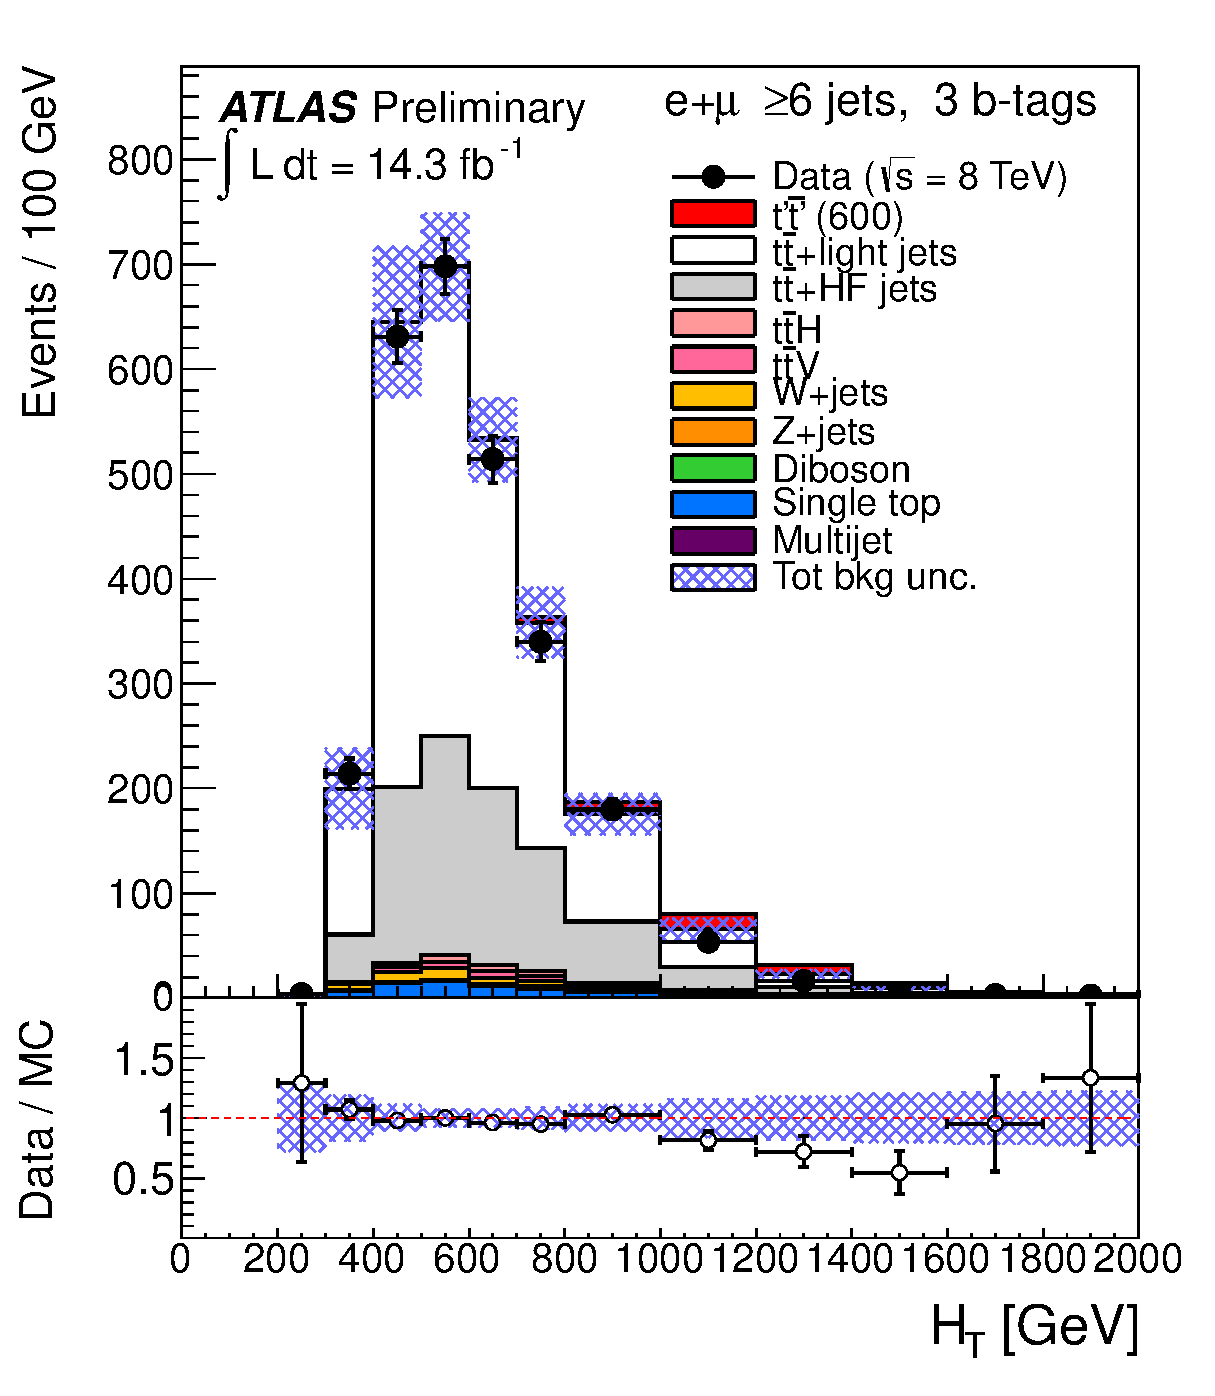
\includegraphics[width=0.45\textwidth]{htx_analysis_14ifb/figures/final/HTAll_6jetin3btagex_ELEMUON.eps}}
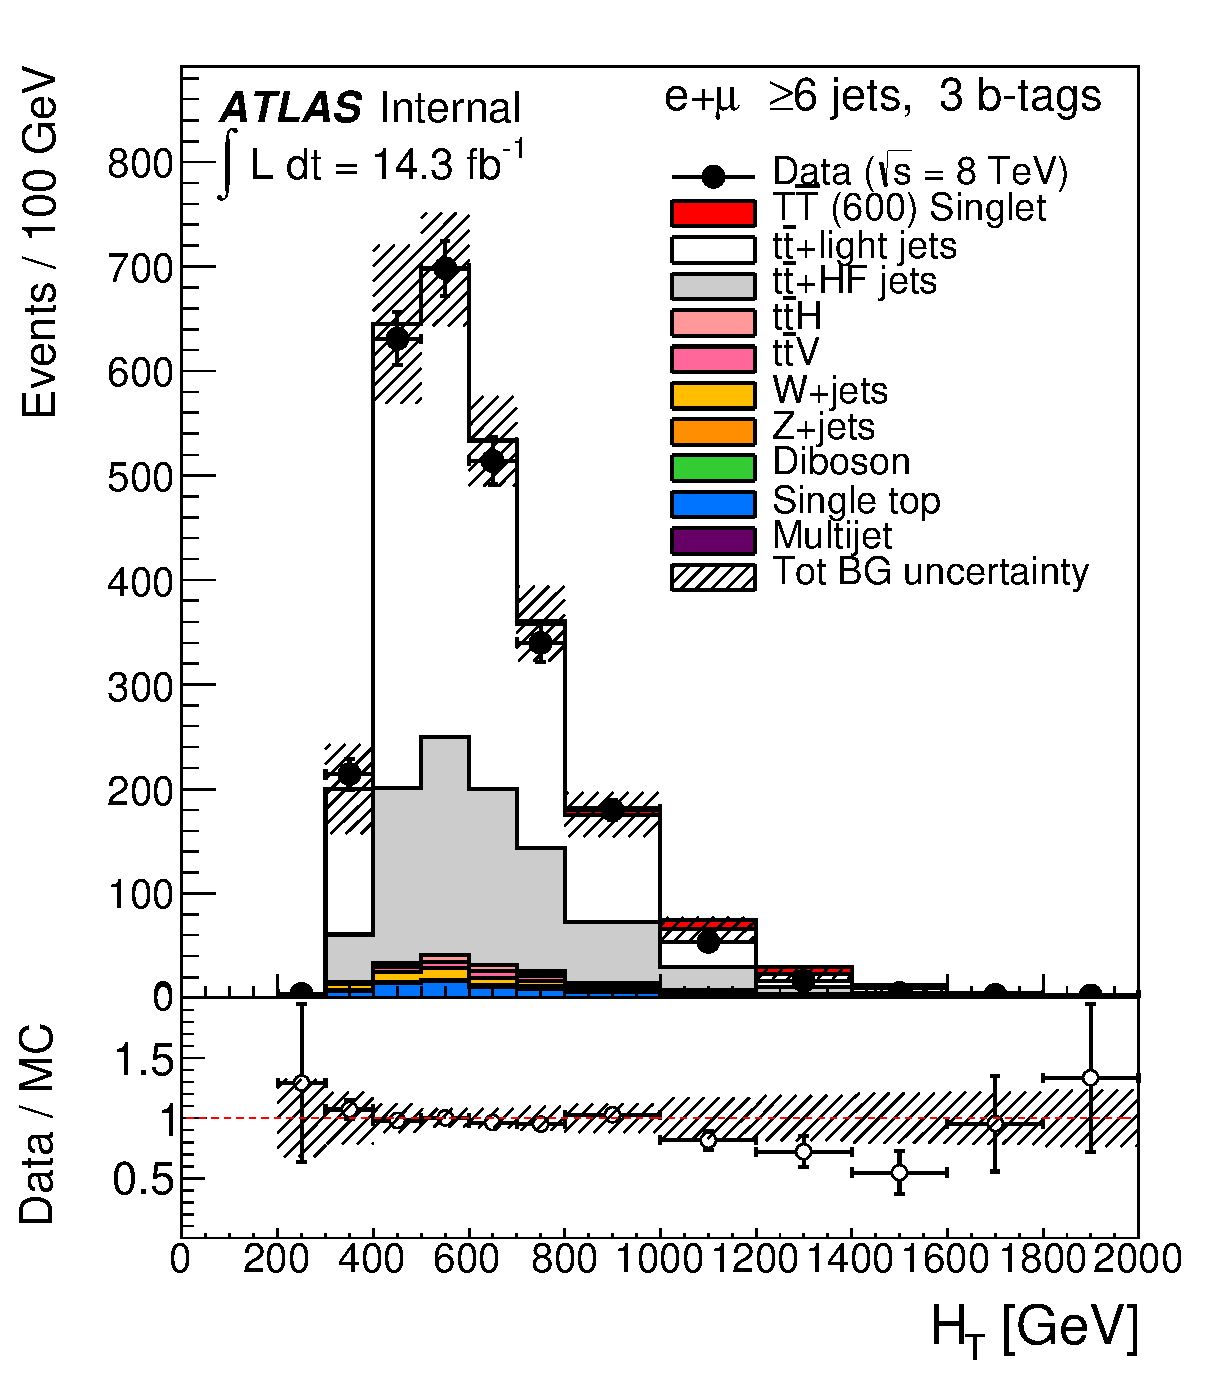
\includegraphics[width=0.45\textwidth]{results/figures/THESIS_c8_signal/HTAll_6jetin3btagex_ELEMUON.eps}}
	\subfigure[]{\label{fig:htx4}
%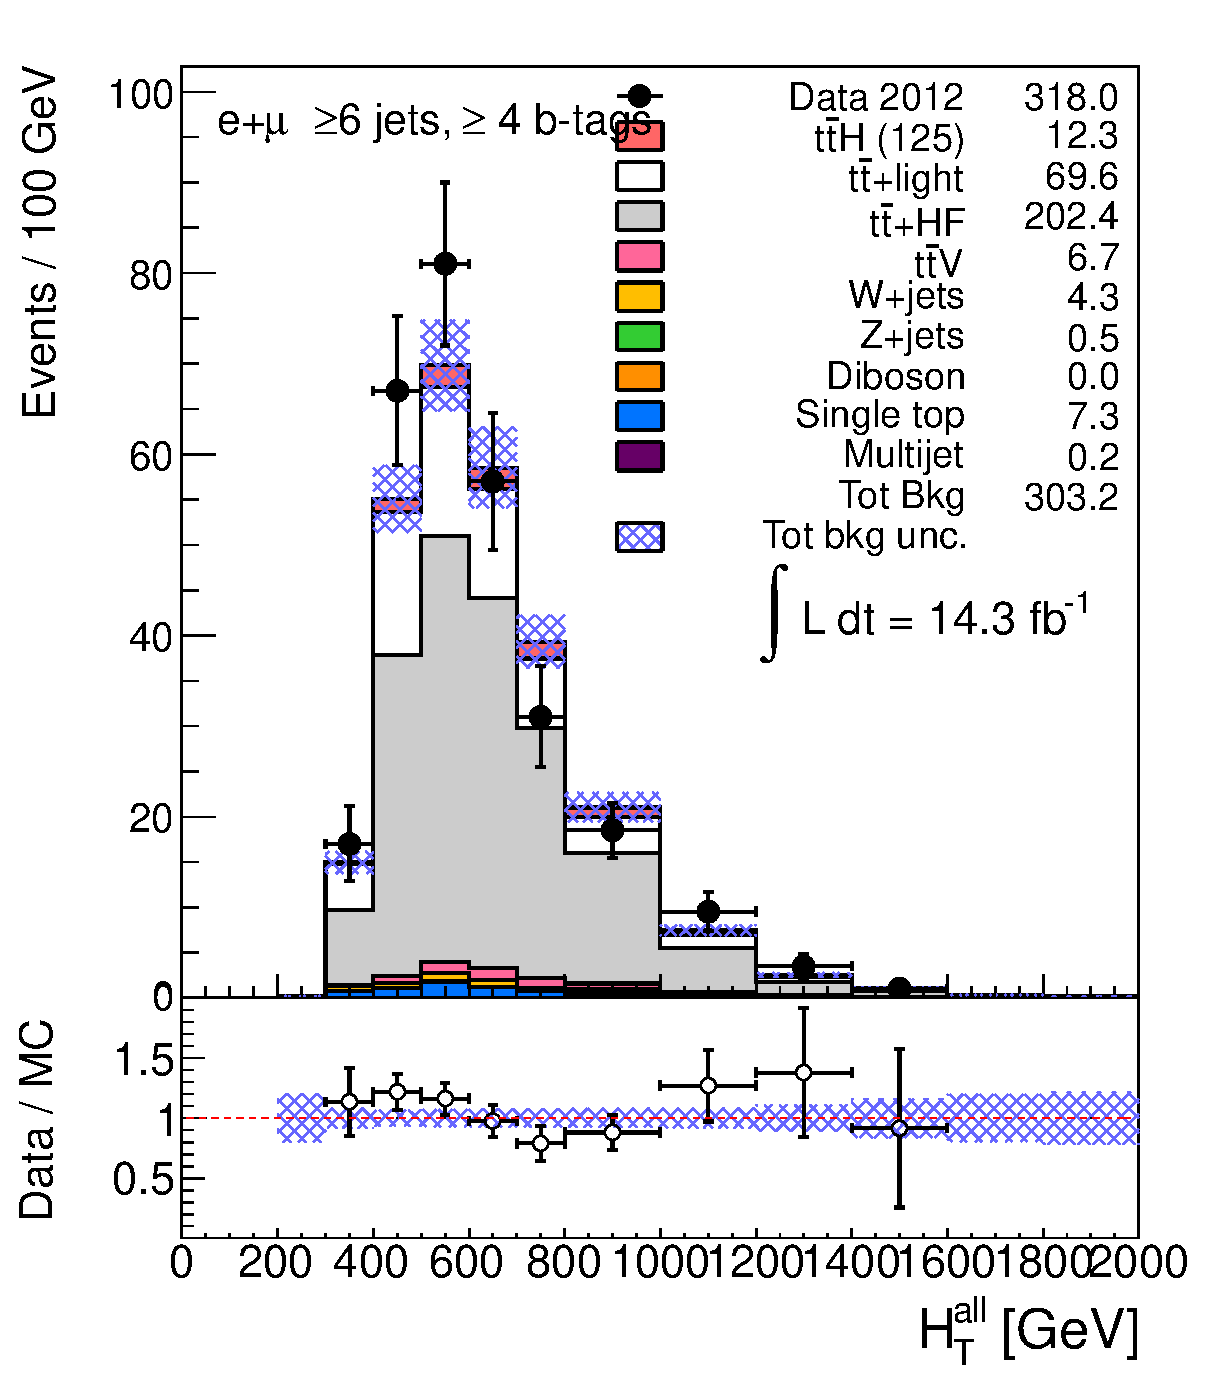
\includegraphics[width=0.45\textwidth]{htx_analysis_14ifb/figures/final/HTAll_6jetin4btagin_ELEMUON.eps}}
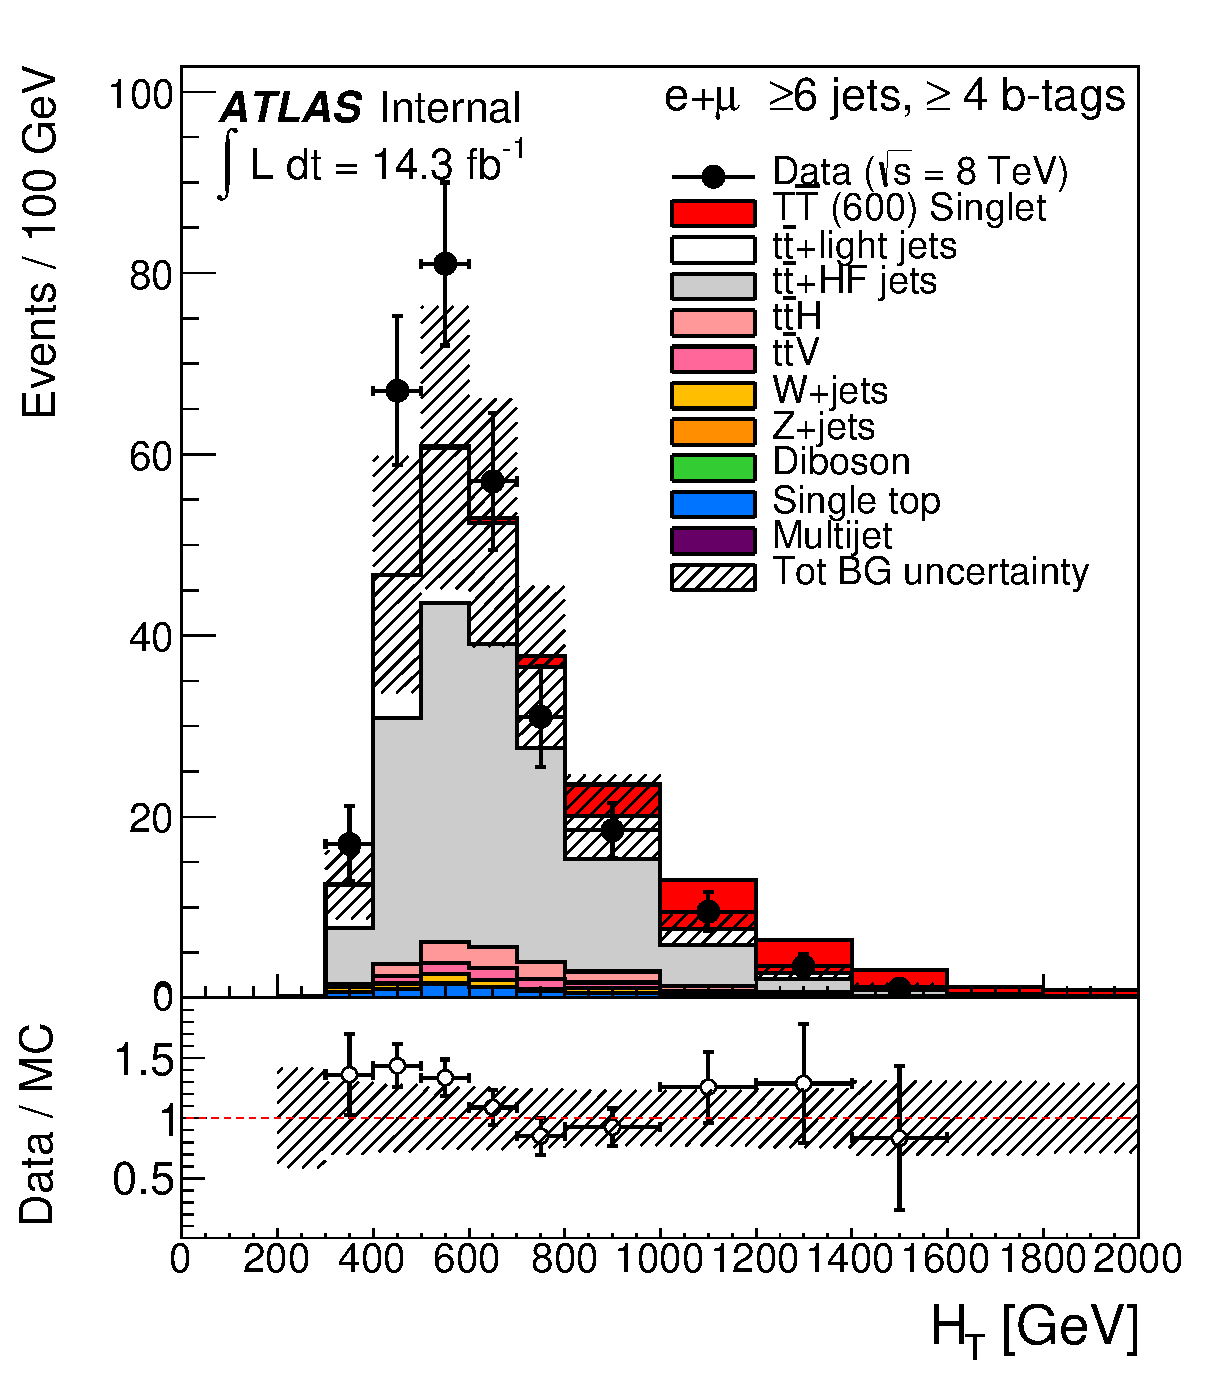
\includegraphics[width=0.45\textwidth]{results/figures/THESIS_c8_signal/HTAll_6jetin4btagin_ELEMUON.eps}}
	\subfigure[]{\label{fig:wbx1}
%\includegraphics[width=0.45\textwidth]{wbx_analysis_14ifb/figures/confnoteplots/VLQAna_WbX_1W_MWb_4_ELEMUON_cutflow1234567_NOMINAL.eps}}
\includegraphics[width=0.45\textwidth]{results/figures/THESIS_c8_signal/VLQAna_WbX_1W_MWb_4_ELEMUON_cutflow1234567_NOMINAL.eps}}
	\caption{Final discriminant variables distributions in the search channels
        of the \htx\ analysis ($\HT$ in (a) \chii, (b) \chiii\ and (c) \chiv\ channels)
        and of the \wbx\ analysis (\mreco\ in the \tight\ channel). In all plots the
        signal is shown for the singlet model. The uncertainty bands include statistical 
        and systematic uncertainties.\label{fig:searchchan}}
\end{center}\end{figure}

For the purpose of a combined statistical analysis
of the four channels,
choices on the systematic 
uncertainties treatment have to be done.
Uncertainties that are common to both analyses and that
are treated in the same way are considered as fully 
correlated and are: integrated luminosity; lepton reconstruction, 
identification and trigger (1 component); jet vertex fraction;
jet energy resolution;
$b$ tagging (9 components); $c$ tagging (5 components); light-jet 
tagging (1 component);
background cross sections ($t\bar{t}$, single top, diboson, $t\bar{t}V$).
For the JES uncertainty, while the \wbx\ analysis considers a single component
the \htx\ uses the 8 components breakdown and is then impossible to 
correlate the individual JES uncertainty sources one by one.
Since in the \htx\ analysis the dominant JES uncertainty eigenvector is the BASELINE
(see Section~\ref{sec:htxSYS}) the choice is to correlate the \wbx\ analysis JES 
uncertainty with the BASELINE uncertainty of the \htx\ analysis.
The systematic uncertainties that are not taken as correlated are:
$W$+jets normalization, divided into 5 components in the \wbx\ 
analysis and only 1 in the \htx\ analysis where, however, is a negligible 
background; $t\bar{t}$ modeling, as the two analyses use different $t\bar{t}$ 
Monte Carlo generators and probe very different
final state kinematics region with different flavor composition.

The benchmark model chosen to show the exclusion limit as a function
of the mass is the vector-like singlet $T$ quark scenario, as
it is the common benchmark model for the two analyses. In this
case the \htx\ analysis performed better than the \wbx\ analysis,
giving an  observed (expected) 95\%  CL  limit value of
$m_{\T}>640\,(615)\gev$.
Figure~\ref{fig:limits1D_combo} shows the observed and expected 
upper limits on the \TTbar\ production cross section 
times branching fraction as a function of $m_{\T}$ for a weak-isospin
singlet  after combination of the two analyses.
The observed (expected) 95\% CL limit is 
$m_{\T}>670\,(675)\gev$ for the central value 
of the theoretical cross section,
improving by $\sim$30$\gev$ the expected sensitivity 
obtained by the \htx\ analysis alone.

\begin{figure}[h!tb]
\centering
\includegraphics[width=0.45\textwidth]{results/figures/lim_singlet_comb.eps} 
\caption[bla]{Observed (solid line) and expected (dashed line) 95\% CL upper limit on the $\T \bar{\T}$ cross section times branching fraction
for a vector-like singlet $\T$ quark  as a function of the $\T$ quark mass, resulting from the combination of
the \wbx\ and the \htx\ analyses.
The surrounding shaded bands correspond to the $\pm1$ and $\pm2$ standard deviations around the expected limit. 
The thin red line and band show the theoretical prediction and its $\pm1$ standard deviation uncertainty.

\label{fig:limits1D_combo}}
\end{figure}

Figure~\ref{fig:limits2D_combo} shows the two-dimensional BR plane for 
different values of $m_{\T}$ with the  resulting 95\% CL exclusion limits.
Comparing this result with the ones of Figures~\ref{fig:limits2D_wbx} 
and~\ref{fig:limits2D_htx} it is evident the improvement resulting
from the combination of the two analyses, covering a much larger
area than the simple addition of two individual ones.
From this picture, vector-like top partners are completely excluded
no matter of the model in the mass range from 350~\gev\ up to 550~\gev\ 
(almost up to 600~\gev).

\begin{figure}[h!bt]
\centering
\includegraphics[width=0.9\textwidth]{results/figures/lim_Scan2D_comb.eps}
\caption{
Observed (red filled area) and expected (red dashed line) 95\% CL exclusion in the plane of
$BR(\T \to Wb)$ versus $BR(\T \to Ht)$, for different values of the vector-like $\T$ quark mass.
The grey (dark shaded) area corresponds to the unphysical region where the sum of branching ratios exceeds unity. 
The default branching ratio values from the \texttt{PROTOS} event generator for the weak-isospin singlet and doublet cases 
are shown as plain circle and star symbols, respectively. This result  from the combination of
the \wbx\ and \htx\ analyses includes both statistical and systematic uncertainties.
\label{fig:limits2D_combo}}
\end{figure}

It is interesting to compare the 
combined result
of the \wbx\ and \htx\ analyses
of Figure~\ref{fig:limits2D_combo} 
with the separate analysis results
to understand the impact on sensitivity
of the statistical combination of
the search channels.
This comparison is presented in 
Figure~\ref{fig:limits2D_potentialcombo},
where the combined result is overlapped
to the two separate results in the BR
plane.
Looking e.g. at the 650~\gev\ mass point,
it can be clearly seen how the singlet
scenario, lying outside of the expected exclusion
region in the case of the single \htx\ analysis,
is then swallowed in the exluded area when
the same analysis is combined with the
\wbx\ analysis, which alone does not even
reach the proximities of that benchmark point.


\begin{figure}[h!bt]
\centering
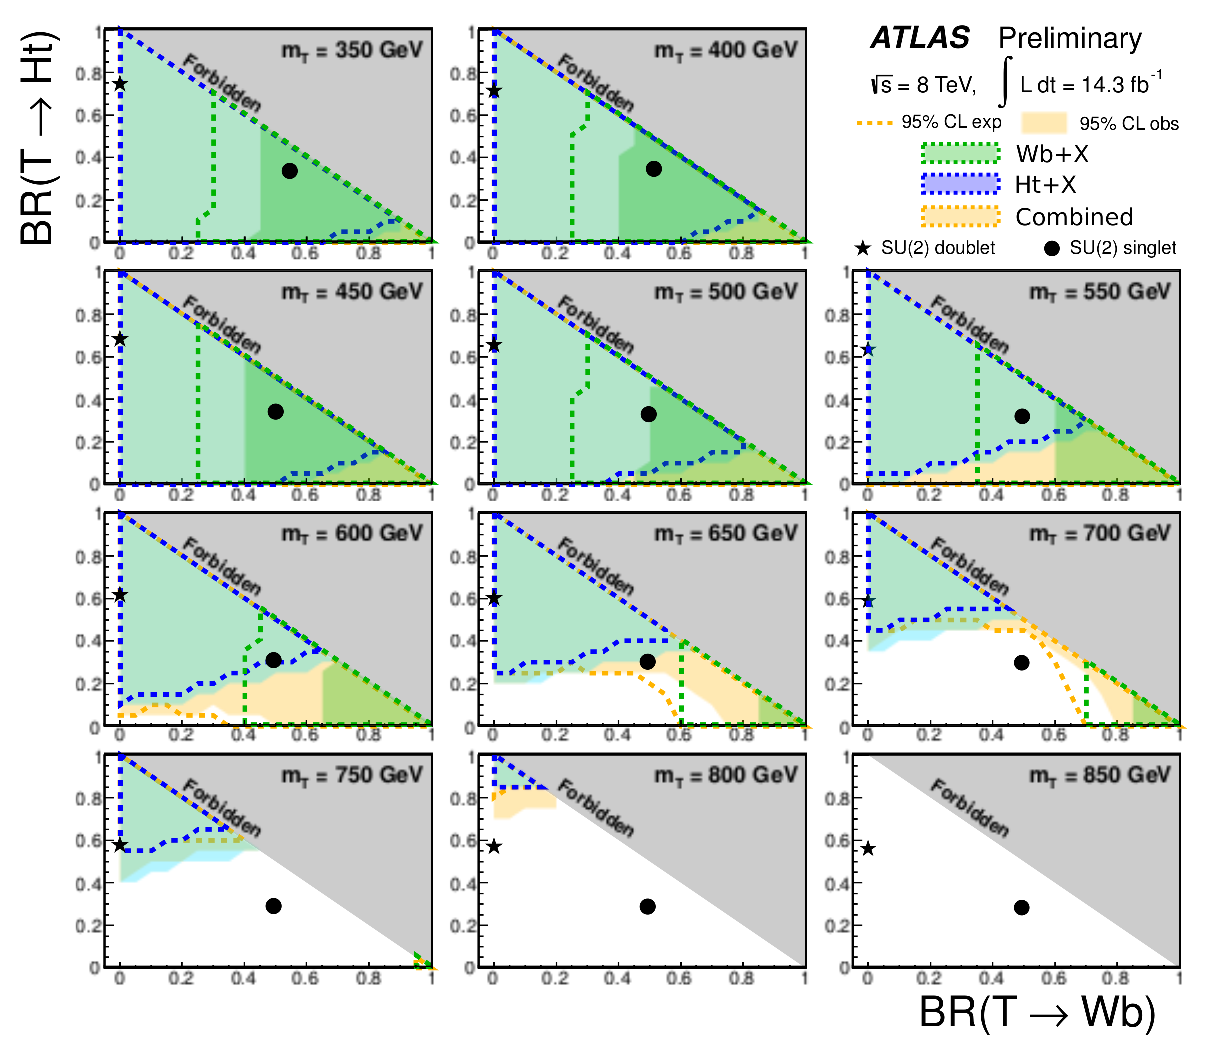
\includegraphics[width=0.9\textwidth]{results/figures/combinationoverlap.eps}
\caption{
Observed (filled area) and expected (dashed line) 95\% CL exclusion in the plane of
$BR(\T \to Wb)$ versus $BR(\T \to Ht)$, for different values of the $\T$ quark mass,
as result of the \wbx\ analysis (green), \htx\ analysis (blue), and the combination of the two (yellow).
The grey (dark shaded) area corresponds to the unphysical region where the sum of branching ratios exceeds unity. 
The default branching ratio values from the \texttt{PROTOS} event generator for the weak-isospin singlet and doublet cases 
are shown as plain circle and star symbols, respectively. All results
include both statistical and systematic uncertainties.
\label{fig:limits2D_potentialcombo}}
\end{figure}

\section{Comparison to other searches}\label{sec:coverage}

As briefly introduced in Section~\ref{sec:strategy}, two
additional analyses have been performed on the same dataset
as the \wbx\ and \htx\ analyses to search for heavy vector-like
top and bottom quarks in final states with exactly two leptons:
a search in the same-sign 
dilepton channel~\cite{ATLAS-CONF-2013-051} and 
a search in the opposite-charge dilepton channel~\cite{ATLAS-CONF-2013-056}.
It was shown that the four analyses probe different 
regions of the 2-dimensional mixing plane and are,
hence, complementary. Even though the single lepton and
the dilepton channels can be considered enough
separated, it was not possible to ensure a complete
orthogonality between all the analyses and they have
not, therefore, been combined\footnote{This
fact is mainly due to the different timescales
and frameworks at which the analyses have been developed. 
The \wbx\ and \htx\ searches
have been conceived to be combined since the
early stages of their design and were performed
inside the same analysis framework.}.
It is however useful to visualize how
the four searches contribute to the full
coverage of the BRs mixing plane by
observing Figure~\ref{fig:limits2D_allcombo}.
Here the results from the four searches,
each obtained independentely, are simply
overlapped. This picture corresponds somehow to
a ``worst case scenario'' of a possible
real combination of the four searches, as
in general the statistical analysis in the
case of additional signal enriched
channels would gain sensitivity. 
This can easily be grasped when looking
at the comparison between the combined result
of the \wbx\ and \htx\ analyses
with the plain overlap of the separate
coverages, shown in the previous section 
in Figure~\ref{fig:limits2D_potentialcombo}.

Figure~\ref{fig:limits2D_allcombo} shows that already
without combining any of the four searches,
\T\ quarks with masses up to 550~\gev, almost up
to 600~\gev, are excluded at 95\% CL without 
any assumption on the model. The same kind of
picture has been obtained in the BR plane for
\B\ quarks, shown in Figure~\ref{fig:limits2D_allvlb}.
Here the analyses contributing to the
95\% CL exclusion in the BR($B\to Hb$) vs  BR($B\to Wt$)
plane are the two searches in the multilepton channel.
The absence of a search probing the top-left corner
of the BR plane leaves for \B\ masses from 400~\gev up to
600~\gev only a very small area uncovered.


\begin{landscape}
\begin{figure}[h!bt]
\centering
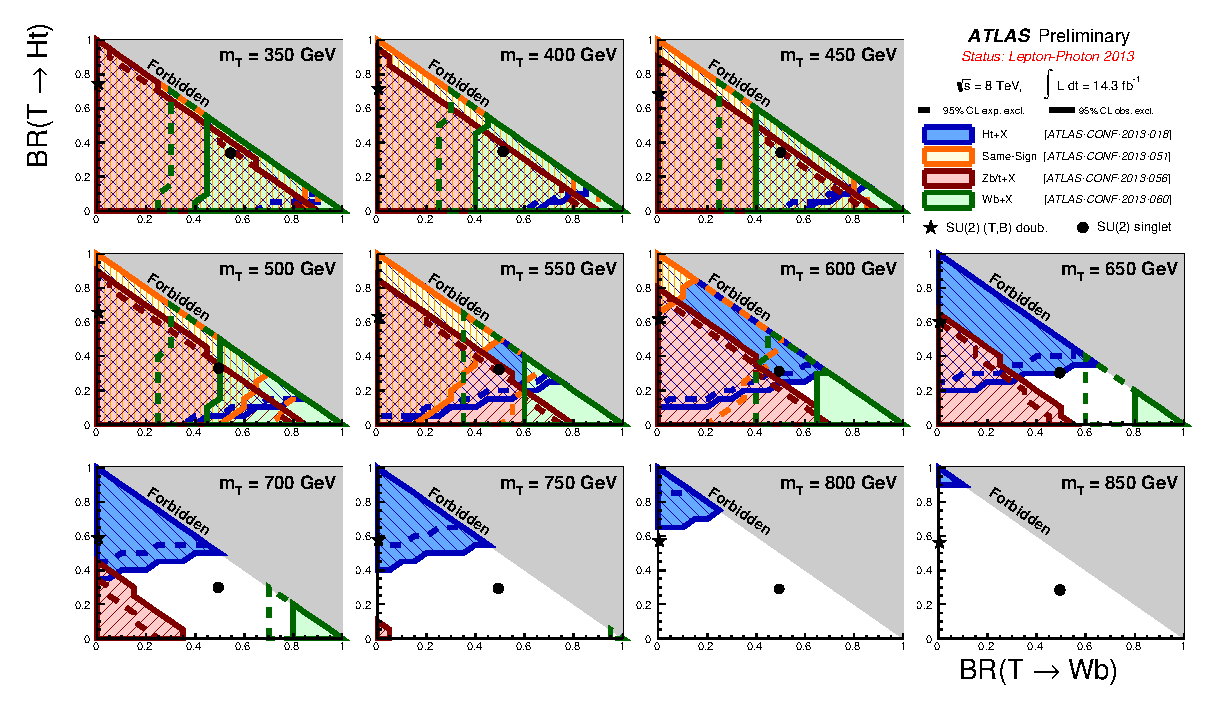
\includegraphics[width=1.5\textwidth]{results/figures/ATLAS_VLQ_TT_june2013_step4.eps}
\caption{
Observed (filled area) and expected (dashed line) 95\% CL exclusion in the plane of
$BR(\T \to Wb)$ versus $BR(\T \to Ht)$, for different values of the $\T$ quark mass.
In blue is shown the area excluded by the single lepton \htx\ analysis;
in orange is shown the area excluded by the same-sign dilepton analysis;
in red is shown the area excluded by the opposite-sign dilepton $\TTbar\to Zt+X$ analysis;
in green is shown the area excluded by the single lepton \wbx\ analysis.
The grey (dark shaded) area corresponds to the unphysical region where the sum of branching ratios exceeds unity. 
The default branching ratio values from the \texttt{PROTOS} event generator for the weak-isospin singlet and doublet cases 
are shown as plain circle and star symbols, respectively. This result includes both statistical and systematic uncertainties.
\label{fig:limits2D_allcombo}}
\end{figure}
\end{landscape}


\begin{landscape}
\begin{figure}[h!bt]
\centering
\includegraphics[width=1.5\textwidth]{results/figures/ATLAS_VLQ_BB_june2013_step2.eps}
\caption{
Observed (filled area) and expected (dashed line) 95\% CL exclusion in the plane of
$BR(\B \to Wt)$ versus $BR(\B \to Hb)$, for different values of the $\B$ quark mass.
In orange is shown the area excluded by the same-sign dilepton analysis;
in red is shown the area excluded by the opposite-sign dilepton $\TTbar\to Zt+X$ analysis.
The grey (dark shaded) area corresponds to the unphysical region where the sum of branching ratios exceeds unity. 
The default branching ratio values from the \texttt{PROTOS} event generator for the weak-isospin singlet and doublet cases 
are shown as plain circle and star symbols, respectively. This result includes both statistical and systematic uncertainties.
\label{fig:limits2D_allvlb}}
\end{figure}
\end{landscape}



\section{Outlook}\label{sec:combOUT}

At the time this dissertation is being
written, all of the four searches for
vector-like quarks are being updated to
the full available statistics of
pp collisions at \rts=8~\tev, about 20~\ifb,
for publication. The four searches maintain the
core strategies but have improvements in
background modeling (in particular with better
and more statistically populated Monte Carlo samples)
and reduced systematic uncertainties.
Searches in new channels are being developed, namely
$B\to Wt+X$ and $B\to Hb+X$, thus allowing for
the full coverage of the BR plane corners.
The complete plan for vector-like quark searches
in ATLAS is to combine all these analyses to 
achieve the highest sensitivity available.


\clearpage{\pagestyle{empty}\cleardoublepage}

\phantomsection
\addcontentsline{toc}{chapter}{Conclusions}
\clearpage{\pagestyle{empty}\cleardoublepage}

\chapter*{Conclusions and outlook}\label{chap:conclusions}

\vskip-1.5cm

Two quasi-model independent searches for 
pair production of vector-like top partners 
in proton-proton collisions at a \cme\ of 8~\tev\ 
have been presented in this dissertation. The final states considered
for both analyses involve one lepton and many jets but different
strategies are adopted in order to achieve sensitivities in different
corners of the decay phase space. Indeed, a peculiar fact for these
searches that has been stressed many times over these pages is the 
unpredicted nature of the heavy vector-like top partners model. 
As a direct consequence, the two analyses have been designed
and developed to be optimized for a particular decay mode and
to have orthogonal channels in order to allow
for a combined search that could exploit the specific sensitivities.

Three particular models, interesting from a theoretical point
of view (but not for this more favoured than others), are considered
over the two analyses: the chiral fourth-generation, with 
BR$(T\to Wb)=1$ for any value of the heavy quark mass; 
the singlet vector-like, with BR$(T\to Wb)\sim 0.5$ and 
BR$(T\to Ht)\sim 0.3$ for almost all
values of the heavy quark mass considered in the searches;
the doublet vector-like, with BR$(T\to Wb)= 0$ and 
BR$(T\to Ht)\in$ [0.50, 0.75] for all the values of the heavy quark mass.
In the \wbx\ analysis, it was possible to exclude at a 95\% CL
pair-produced chiral fourth-generation top partners and vector-like
$Y$ quarks with masses up to 740~\gev, and pair-produced vector-like 
singlet top partners with  masses up to 505~\gev.
In the \htx\ analysis, it was possible to exclude at a 95\% CL
pair-produced vector-like singlet and doublet top partners with 
masses up to 640~\gev\ and 790~\gev\ respectively.
When the two analyses are combined, the observed exclusion limit
for the only model where both analyses are sensitive, the
vector-like singlet $T$, is pushed $\sim$30~\gev\ further the
best result of the two, obtained by the \htx\ analysis,
achieving a 95\% CL exclusion of pair-produced vector-like singlet 
top partners with masses up to 670~\gev. While this might not
look like a significant improvement, the power of the combination
of the two searches is evident looking at the coverage of the
two-dimensional branching ratio plane, where  95\% CL exclusion is set for
pair-produced vector-like top partners with masses up to 550~\gev\ 
independently from the model, and also the plane for the 600~\gev\ mass
point is almost fully excluded. This strongly encourages to perform,
in the future, full combination of searches for vector-like quarks.

The mass range excluded at 95\% CL up to now
is getting closer and closer to the point where pair-production
of vector-like quarks will start to be disfavoured with respect
to single production. In this sense, while it is desirable to continue to
exploit the experience achieved up to now with the searches for
pair-produced vector-like quarks in the single lepton and multi-lepton
channels, it is a good idea to start designing searches for
single-produced vector-like quarks for LHC Phase-II.
Further improvements are possible for the searches
presented in this dissertation without changing the core of
the analysis strategies. During Phase-II they will benefit
of the increased \cme\ available for heavy quark production
in pp collisions with \rts=14~\tev\ and of the high integrated
luminosity (100~\ifb\ of data are expected over three years
of operation). With high luminosity comes the challenge of
dealing with higher pile-up, but considering that vector-like
quark searches involve high-\pt\ objects this should not
represent a major issue.

Besides the great discovery potential, the combination
of multiple searches will provide useful insights on the
exotic quark properties, like their quantum numbers or
the measurement of their branching ratios. 
Adding searches for single production of vector-like quarks
would also allow to measure the electroweak couplings of
these particles with the Standard Model quarks from the third generation.
Finally, these searches are even more interesting since
they will probe a wide range of
signatures that are often shared with other new physics
scenarios. Given the fact that during these last successful years
of LHC operation no hints on what lies ``beyond the Standard Model''
have emerged, the winning strategy is for sure not to confine ourselves 
to exclusive models.


\clearpage{\pagestyle{empty}\cleardoublepage}

\appendix

\clearpage{\pagestyle{empty}\cleardoublepage}

\chapter{}\label{appA:}


\clearpage{\pagestyle{empty}\cleardoublepage}

\clearpage{\pagestyle{empty}\cleardoublepage}

\chapter{}\label{appB:}


\clearpage{\pagestyle{empty}\cleardoublepage}
\input{wbx_analysis_7tev/wbx7tev}

%\clearpage{\pagestyle{empty}\cleardoublepage}
%\clearpage{\pagestyle{empty}\cleardoublepage}

\chapter{Preliminary search  for \TTbar\ pairs decaying to $Ht+X$}\label{chap:htx}

\section{Control regions}\label{sec:htxCR}

\section{Event selection}\label{sec:htxEVT}

%\section{}\label{sec:}

%\section{}\label{sec:}

\section{Systematics}\label{sec:htxSYS}



%%%%NB COPY PASTE
The total prior systematic uncertainty
in the background normalisation in the $\geq 4$ $b$-tags channel is 
$\sim$42\%, with the dominant uncertainties being from $b$ tagging efficiency (16\%),
$c$ tagging efficiency (11\%), jet energy scale (11\%), $t\bar{t}$ modelling (11\%), 
$t\bar{t}$+heavy-flavour fractions (32\%) and $t\bar{t}$ cross section (10\%).
As a result of the two-parameter fit, the total background uncertainty is reduced 
by about 80\% in this channel. The total  systematic uncertainty
in the signal normalisation in the $\geq 4$ $b$-tags channel is 
$\sim$21\%, completely dominated by the uncertainty in the $b$ tagging efficiency.


%\phantomsection
%\addcontentsline{toc}{chapter}{Ringraziamenti}
%\input{smallstuff/ringraziamenti}

\clearpage{\pagestyle{empty}\cleardoublepage}


\backmatter

%\nocite{}
\phantomsection
\addcontentsline{toc}{chapter}{Bibliography}

%\bibliographystyle{woc}
%\bibliographystyle{unsrt}
\bibliographystyle{bibliography/atlasnote}
\bibliography{bibliography/biblio}

\clearpage{\pagestyle{empty}\cleardoublepage}



\end{document}
